% --------------------------------------------------------------
% This is all preamble stuff that you don't have to worry about.
% Head down to where it says "Start here"
% --------------------------------------------------------------
 
\documentclass[english]{article}

 
\usepackage[margin=1in]{geometry} 
\usepackage{amsmath,amsthm,amssymb}
\usepackage{graphicx}
\usepackage{float}
\usepackage{listings}
\usepackage{babel,blindtext}

\newcommand{\N}{\mathbb{N}}
\newcommand{\Z}{\mathbb{Z}}
%\usepackage[]{mcode}
   
\usepackage{graphicx}
\pagestyle{empty}

\newcommand*\colvec[3][]{
    \begin{pmatrix}\ifx\relax#1\relax\else#1\\\fi#2\\#3\end{pmatrix}
}
 
\begin{document}
 
% --------------------------------------------------------------
%                         Start here
% --------------------------------------------------------------
 
%\renewcommand{\qedsymbol}{\filledbox}
 
\title{Wavelet Fractal Transform}%replace X with the appropriate number
\author{Stanislav Zonov ~ \\ %replace with your name
AMATH 495} %if necessary, replace with your course title
 
\maketitle
\newpage


\newpage
\section{lenna.pnm}
\begin{figure}[H]
	\centering
  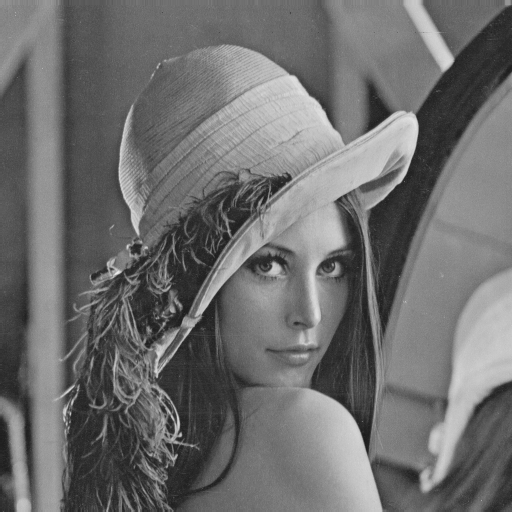
\includegraphics[width=.5\linewidth]{../images/lenna.png}
  \label{fig:fig1}
  \caption{Original.}
\end{figure}

\begin{figure}[!htb]
\minipage{0.32\textwidth}
  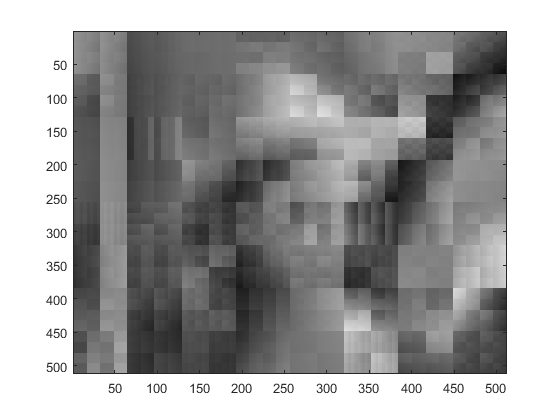
\includegraphics[width=\linewidth]{lenna/lenna_approx.png}
  \caption{6 levels}\label{fig:awesome_image1}
\endminipage\hfill
\minipage{0.32\textwidth}
  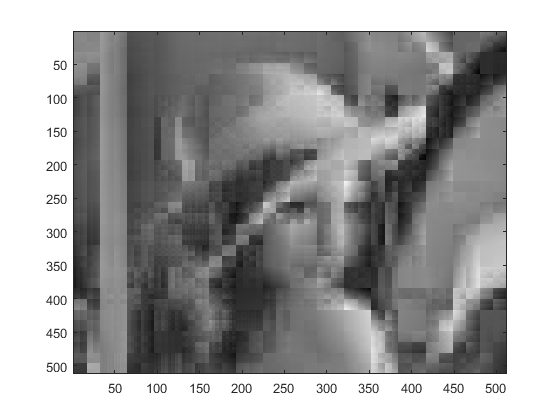
\includegraphics[width=\linewidth]{lenna/lenna_approx_2.png}
  \caption{5 levels}\label{fig:awesome_image2}
\endminipage\hfill
\minipage{0.32\textwidth}%
  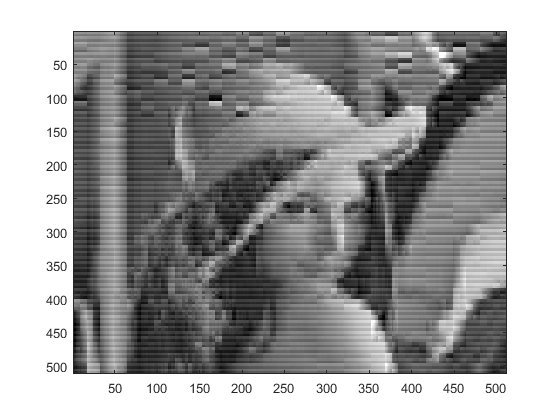
\includegraphics[width=\linewidth]{lenna/lenna_approx_3.png}
  \caption{4 levels}\label{fig:awesome_image3}
\endminipage
\end{figure}



\newpage
\section{boat.pnm}
\begin{figure}[H]
	\centering
  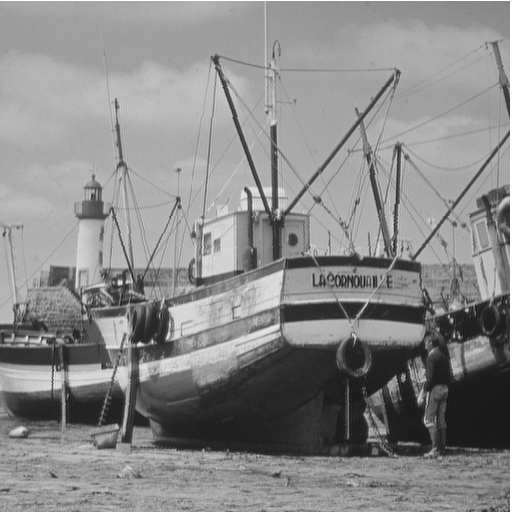
\includegraphics[width=.5\linewidth]{../images/boat.png}
  \label{fig:fig1}
  \caption{Original.}
\end{figure}

\begin{figure}[!htb]
\minipage{0.32\textwidth}
  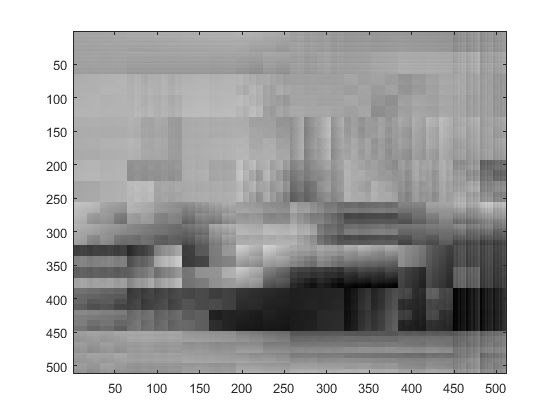
\includegraphics[width=\linewidth]{boat/boat_approx.png}
  \caption{6 levels}\label{fig:awesome_image1}
\endminipage\hfill
\minipage{0.32\textwidth}
  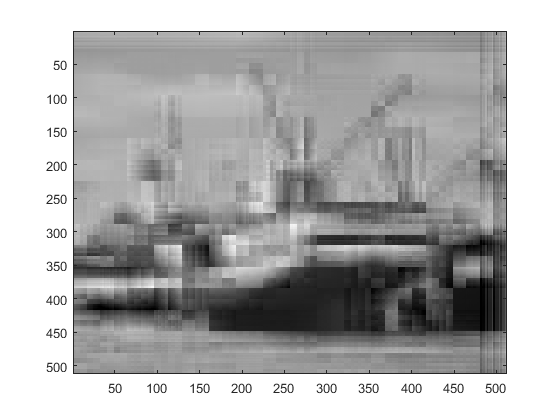
\includegraphics[width=\linewidth]{boat/boat_approx_2.png}
  \caption{5 levels}\label{fig:awesome_image2}
\endminipage\hfill
\minipage{0.32\textwidth}%
  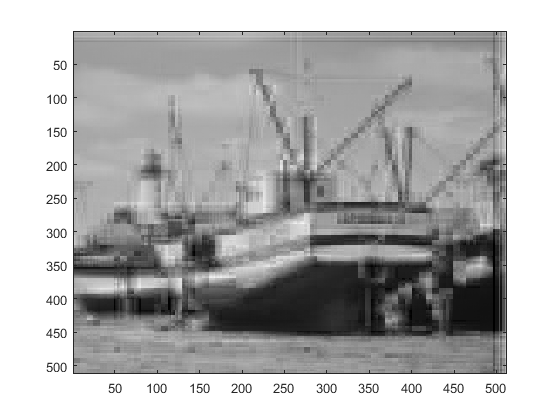
\includegraphics[width=\linewidth]{boat/boat_approx_3.png}
  \caption{4 levels}\label{fig:awesome_image3}
\endminipage
\end{figure}


\newpage
\section{mandrill.pnm}
\begin{figure}[H]
	\centering
  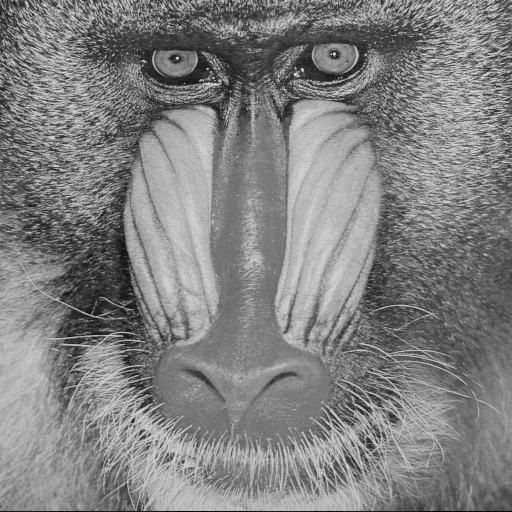
\includegraphics[width=.5\linewidth]{../images/mandrill.png}
  \label{fig:fig1}
  \caption{Original.}
\end{figure}

\begin{figure}[!htb]
\minipage{0.32\textwidth}
  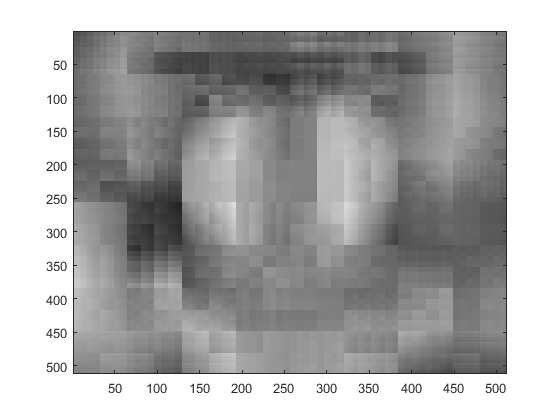
\includegraphics[width=\linewidth]{mandrill/mandrill_approx.png}
  \caption{6 levels}\label{fig:awesome_image1}
\endminipage\hfill
\minipage{0.32\textwidth}
  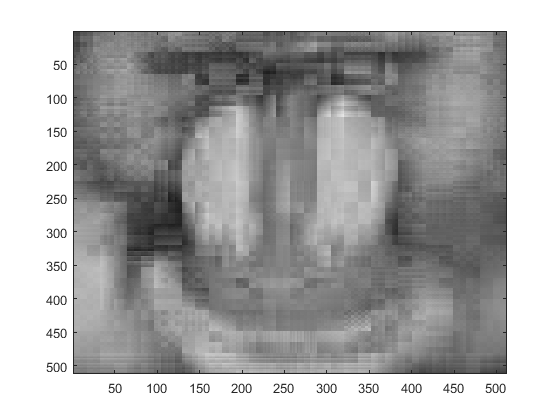
\includegraphics[width=\linewidth]{mandrill/mandrill_approx_2.png}
  \caption{5 levels}\label{fig:awesome_image2}
\endminipage\hfill
\minipage{0.32\textwidth}%
  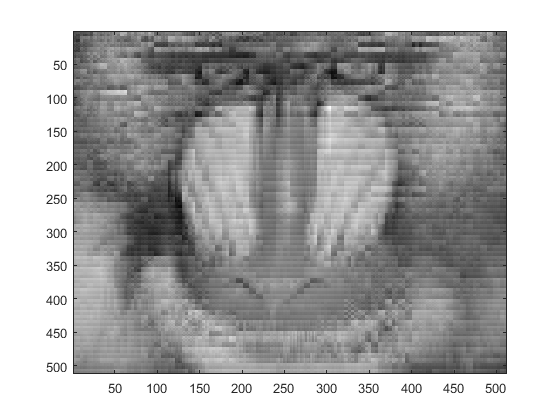
\includegraphics[width=\linewidth]{mandrill/mandrill_approx_3.png}
  \caption{4 levels}\label{fig:awesome_image3}
\endminipage
\end{figure}

\end{document}
